\hypertarget{group___p_i_d}{}\section{P\+ID Motor Control}
\label{group___p_i_d}\index{P\+I\+D Motor Control@{P\+I\+D Motor Control}}
Collaboration diagram for P\+ID Motor Control\+:
\nopagebreak
\begin{figure}[H]
\begin{center}
\leavevmode
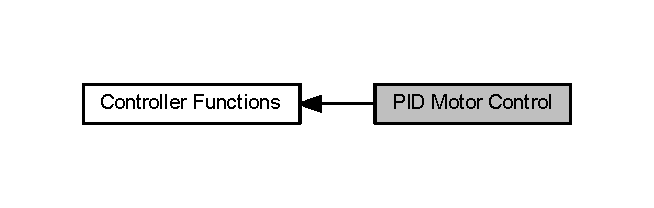
\includegraphics[width=314pt]{group___p_i_d}
\end{center}
\end{figure}


\subsection{Detailed Description}
A Proportional Integral Derivative (P\+ID) controller is a generic feedback control loop mechanism widely used in industrial control systems. A P\+ID controller is the most commonly used type of feedback controller.

This set of functions implements (P\+ID) controllers for Q15, Q31, and floating-\/point data types. The functions operate on a single sample of data and each call to the function returns a single processed value. {\ttfamily S} points to an instance of the P\+ID control data structure. {\ttfamily in} is the input sample value. The functions return the output value.

\begin{DoxyParagraph}{Algorithm\+:}

\begin{DoxyPre}
   y[n] = y[n-1] + A0 * x[n] + A1 * x[n-1] + A2 * x[n-2]
   A0 = Kp + Ki + Kd
   A1 = (-Kp ) - (2 * Kd )
   A2 = Kd  \end{DoxyPre}

\end{DoxyParagraph}
\begin{DoxyParagraph}{}
where {\ttfamily Kp} is proportional constant, {\ttfamily Ki} is Integral constant and {\ttfamily Kd} is Derivative constant
\end{DoxyParagraph}
\begin{DoxyParagraph}{}
 
\end{DoxyParagraph}
\begin{DoxyParagraph}{}
The P\+ID controller calculates an \char`\"{}error\char`\"{} value as the difference between the measured output and the reference input. The controller attempts to minimize the error by adjusting the process control inputs. The proportional value determines the reaction to the current error, the integral value determines the reaction based on the sum of recent errors, and the derivative value determines the reaction based on the rate at which the error has been changing.
\end{DoxyParagraph}
\begin{DoxyParagraph}{Instance Structure}
The Gains A0, A1, A2 and state variables for a P\+ID controller are stored together in an instance data structure. A separate instance structure must be defined for each P\+ID Controller. There are separate instance structure declarations for each of the 3 supported data types.
\end{DoxyParagraph}
\begin{DoxyParagraph}{Reset Functions}
There is also an associated reset function for each data type which clears the state array.
\end{DoxyParagraph}
\begin{DoxyParagraph}{Initialization Functions}
There is also an associated initialization function for each data type. The initialization function performs the following operations\+:
\begin{DoxyItemize}
\item Initializes the Gains A0, A1, A2 from Kp,Ki, Kd gains.
\item Zeros out the values in the state buffer.
\end{DoxyItemize}
\end{DoxyParagraph}
\begin{DoxyParagraph}{}
Instance structure cannot be placed into a const data section and it is recommended to use the initialization function.
\end{DoxyParagraph}
\begin{DoxyParagraph}{Fixed-\/\+Point Behavior}
Care must be taken when using the fixed-\/point versions of the P\+ID Controller functions. In particular, the overflow and saturation behavior of the accumulator used in each function must be considered. Refer to the function specific documentation below for usage guidelines. 
\end{DoxyParagraph}
